%1234567890123456789012345678901234567890123456789012345678901234567890123456789
%         1         2         3         4         5         6         7        8

\documentclass[runningheads,a4paper]{llncs}
\usepackage{amssymb}
\setcounter{tocdepth}{3}
\usepackage{graphicx}
\usepackage{amssymb}
\usepackage[utf8]{inputenc}
\usepackage{url}

% \usepackage{breakurl}
\usepackage{float}
\usepackage{amsmath}
\usepackage{graphicx}
\usepackage[tight]{subfigure}
\usepackage{wrapfig}

\usepackage{lipsum}

\newcommand{\robospecs}{%
  \newpage%
  \pagenumbering{gobble}%
% \pagestyle{fancy}%
% \fancyhf{}%
%  \chead{$|$}
% \rhead{\footnotesize\thetitle}%
% \lhead{\footnotesize\theauthor}%
% \rfoot{Robot software and hardware specification sheet}%
}


\newcommand{\teamori}{Team ORIon}
\newcommand{\competitionyear}{2022}
\newcommand{\competitioncountry}{Thailand}
\newcommand{\robocuptitleshort}{RoboCup \competitionyear}

\usepackage{hyperref}
\hypersetup{
    colorlinks=true,
    linkcolor=black,
    anchorcolor=black,
    urlcolor=black,
    citecolor=black,
    filecolor=black
}
%https://www.youtube.com/watch?v=sZ_oqFDUsnM
\begin{document}

\authorrunning{Ricardo Cannizzaro et al.}

\title{\teamori\ --- 2022 Team Description Paper}

\author{Ricardo Cannizzaro \and Clarissa Costen \and Matthew Budd \and Shu Ishida \and Marc Rigter \and Lars Kunze \and Ioannis Havoutis \and Nick Hawes \and Bruno Lacerda}
\institute{Oxford Robotics Institute, Dept. of Engineering Science, University of Oxford, UK \\
\texttt{orion@oxfordrobotics.institute} \\
\url{https://ori.ox.ac.uk/student-teams/team-orion}}

\maketitle

%%%%%%%%%%%%%%%%%%%%%%%%%%%%%%%%%%%%%%%%%%%%%%%%%%%%%%%%%%%%%%%%%%%%%%%%%%%%%%%%%%%%

\begin{abstract}
This document outlines the approach \textit{\teamori} will take to the RoboCup@Home 2022 (DSPL).
Our first experience competing with Toyota's Human Support Robot (HSR) was at the World Robot Summit (WRS) 2018. We have since competed at RoboCup 2019 in the DSPL @Home league. Due to the coronavirus pandemic, we were unable to compete in the 2020 and 2021 competitions. However, we aim to return to the competition in 2022 with a refreshed team and revamped HSR.
Our research interests are centred around long-term autonomy; mobility and whole body motion planning; causal reasoning and knowledge representation; and trustworthy and explainable AI.
Advances in these directions will enable service robots to interact with humans and complete useful everyday tasks in typical household settings. 
We aim to demonstrate robust and intelligent autonomous behaviour, that uses experience to learn and refine a growing set of robot skills, on the HSR.
\end{abstract}


%%%%%%%%%%%%%%%%%%%%%%%%%%%%%%%%%%%%%%%%%%%%%%%%%%%%%%%%%%%%%%%%%%%%%%%%%%%%%%%%%%%%

%The TDP is an 8-pages (+ annex) long scientific paper, detailing information on the technical and scientific approach of the team's research, while including also the following:
%\begin{itemize}
%	\item \checkmark Innovative technology and scientific contribution
%    \item \checkmark Focus of research/research interests
%    \item \checkmark Re-usability of the system for other research groups
%    \item \checkmark Applicability of the robot in the real world
%	\item \checkmark DSPL and SSPL: When the robot depicted in the TDP or Team Video is different from the league's standard one, the TDP must clearly state how the addressed approach and described software will be adapted to the standard platform robot.
%\end{itemize}


\section{Introduction}

\textit{\teamori{}} is a student robotics competition team created in 2018 within the Oxford Robotics Institute (ORI) at the University of Oxford. 
The team consists of undergraduate and graduate students, and is supported by robotics postdoc researchers, principal investigators, and other faculty members of the ORI. 
We come from a strong research institute with seminal work in mobile autonomy and machine learning. The ORI has a significant track record in field robotics and real-world trials of autonomous systems.
Further, the ORI also has a team of professional hardware and software engineers. This experience and support is leveraged to deliver a strong performance in the RoboCup competition.

\subsection{Past Competition Involvements}
The RoboCup@Home league provides a challenging environment and complex tasks to which new and existing ORI research can be applied.
Since acquiring our Toyota Human Support Robot (HSR) in 2018, we have competed in the Partner Robot Challenge of WRS; we also competed in the 2019 RoboCup@Home competition, placing $6^{th}$ out of 10 on our first attempt at the competition (see Figure~\ref{fig:pastcompetitions}). 
The HSR robot allows us to focus on developing the intelligence required for successfully completing complex tasks, without the added burden of building and maintaining a custom platform.
Competing in the \robocuptitleshort\ event will allow us to demonstrate the capabilities presented in this document and will provide valuable experience for our future participations.

\subsection{Public Outreach}
We also run robot demonstrations to the public at outreach events (e.g., the Goodwood Festival of Speed), to promote greater awareness and interest in STEM, robotics, and AI to the wider public. In October 2019, we demonstrated the HSR for His Royal Highness Prince William at the ORI to celebrate the opening of a new college building (see Figure~\ref{fig:outreach}).

\begin{figure}[tb]
	\begin{center}
  		\includegraphics[width=.41\columnwidth, clip, trim=0 0ex 0ex 50ex]{images/hsr_grasping.jpg}
  		\includegraphics[width=.49\columnwidth, clip, trim=0 0ex 0ex 50ex]{images/robocup_team.jpg}
	\end{center} 
	\caption{\emph{Left:} Team ORIon's HSR grasping a plant at the World Robot Summit (WRS) 2018 in Tokyo, Japan. \emph{Right:} Team ORIon at RoboCup@Home 2019 in Sydney, Australia.}
	\label{fig:pastcompetitions}
\end{figure}

\begin{figure}[tb]
	\begin{center}
		\includegraphics[width=.20\columnwidth, clip, trim=0 0ex 0ex 0ex]{images/goodwood_hsr_coffee.jpg}
		\includegraphics[width=.39\columnwidth, clip, trim=20ex 0ex 0ex 0ex]{images/goodwood_demo_with_child.jpg}
		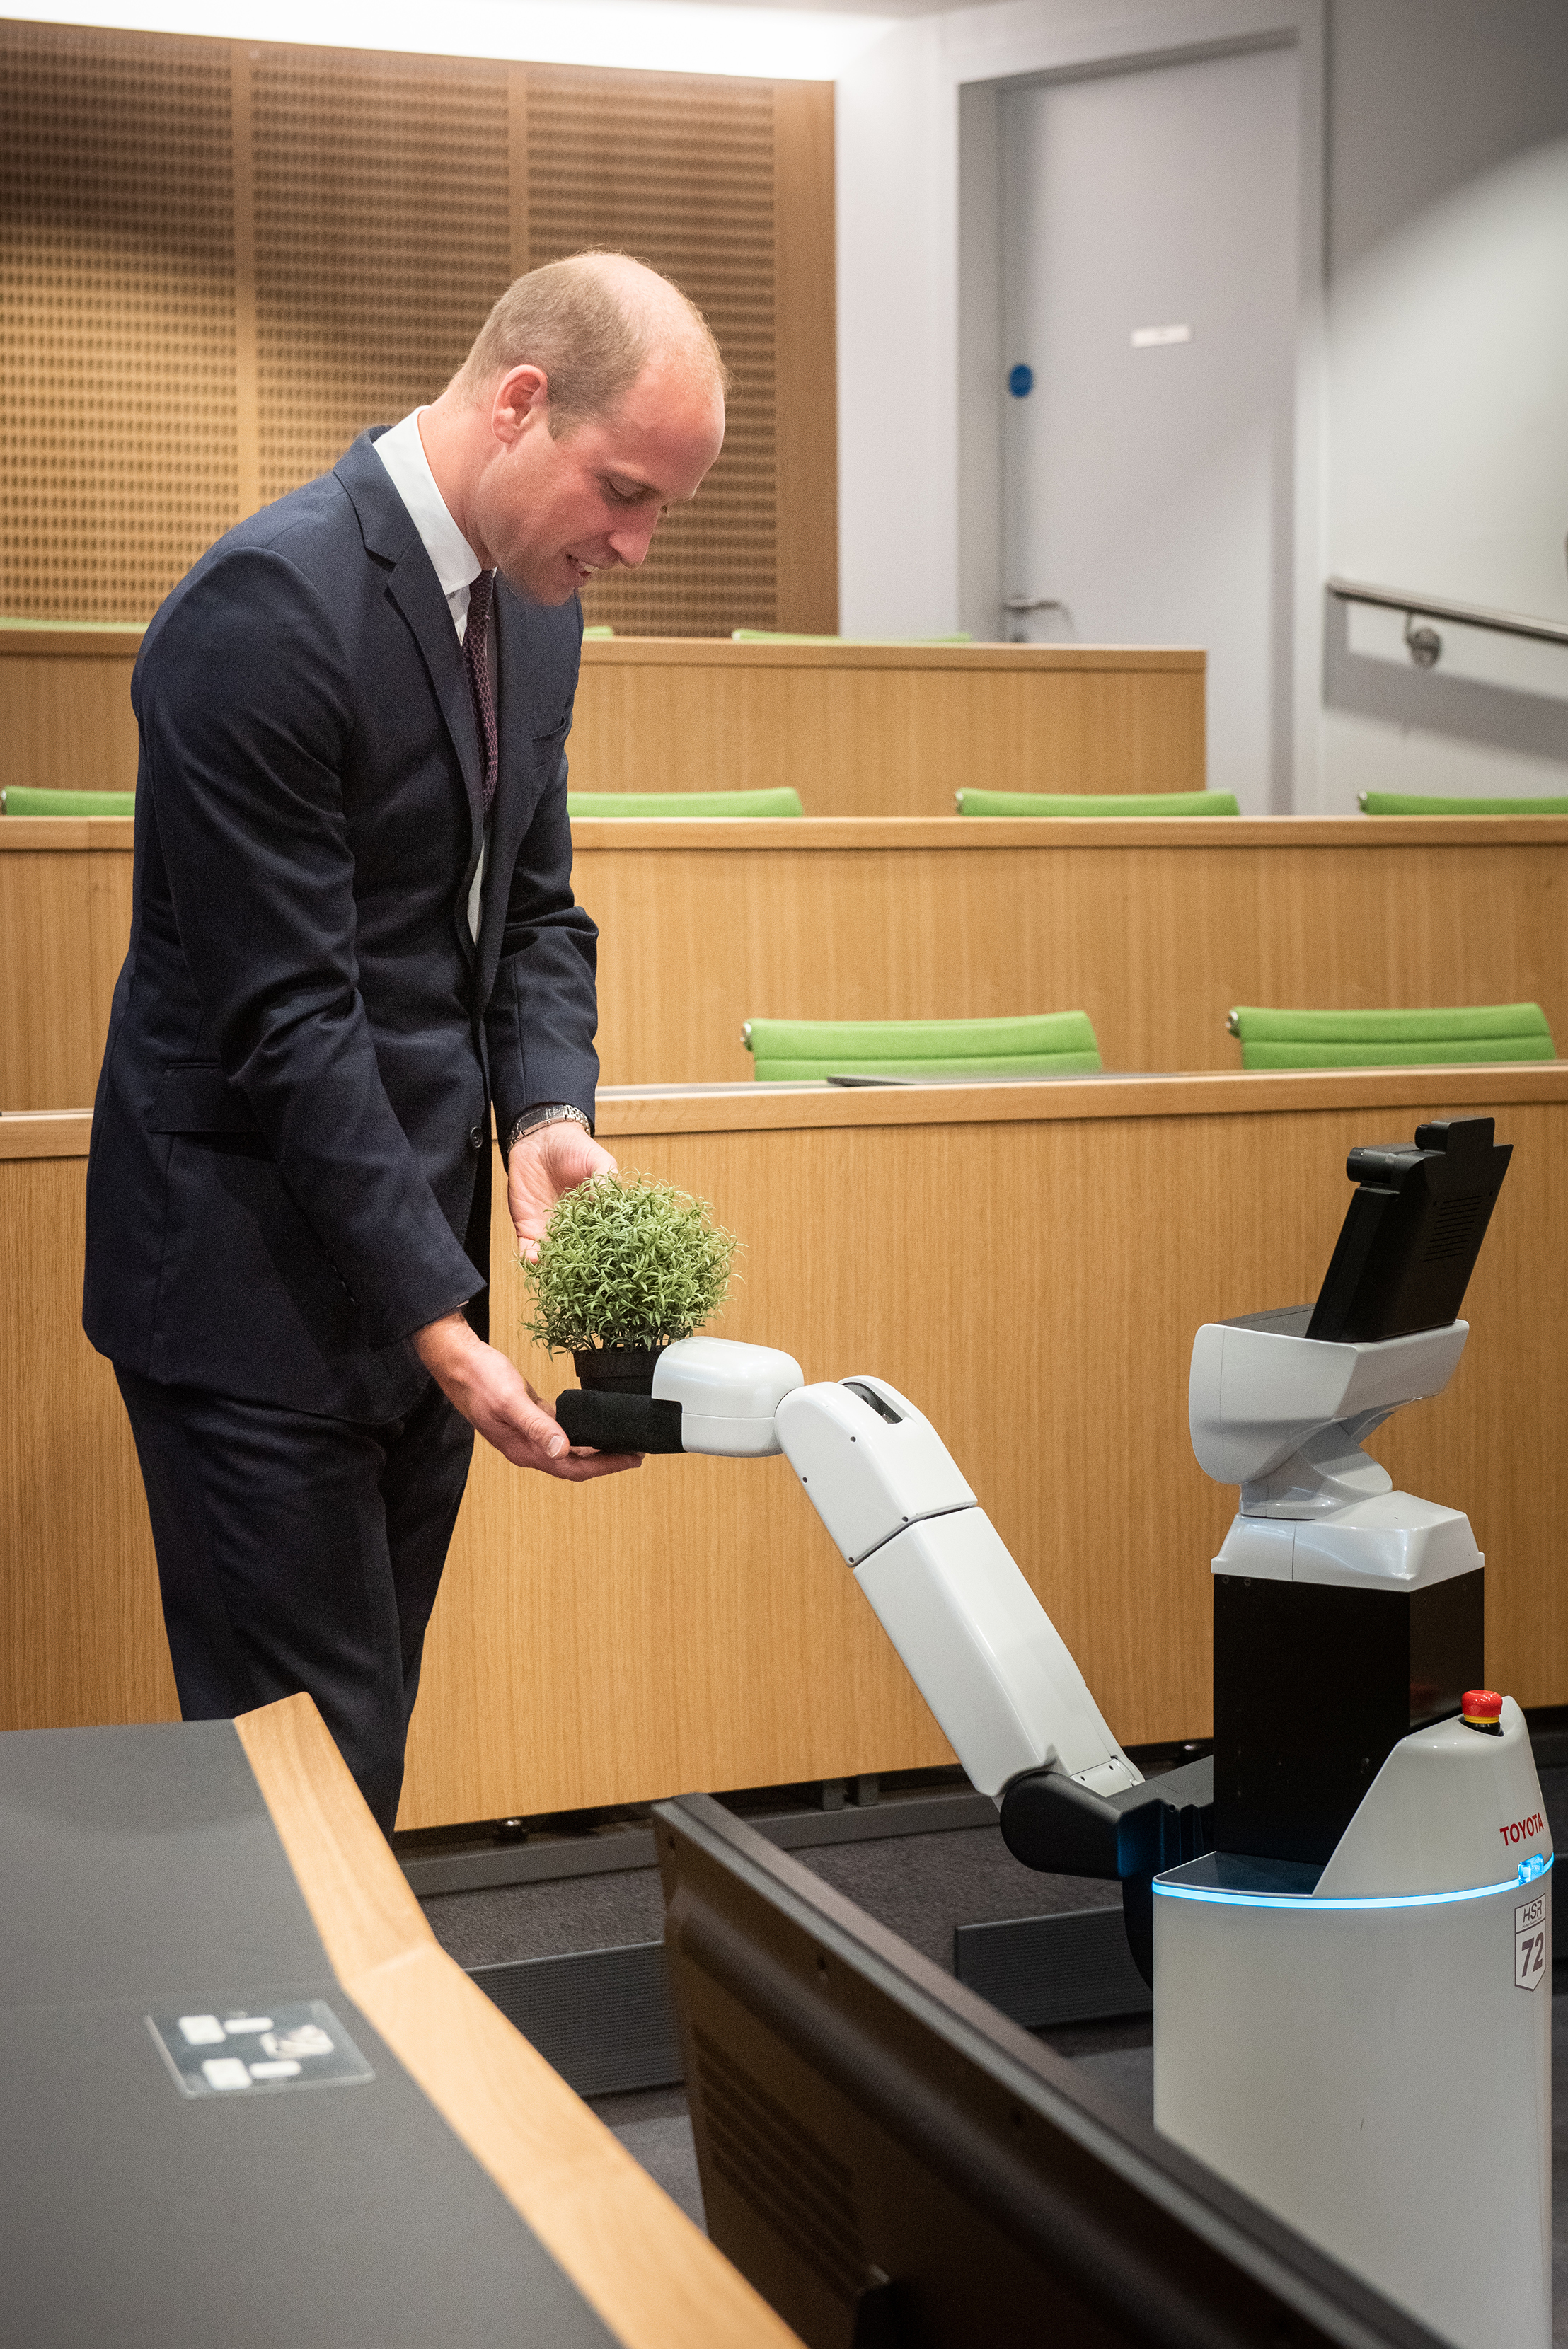
\includegraphics[width=.214\columnwidth, clip, trim=0ex 0ex 0ex 15ex]{images/keble_college_duke_of_cambridge_hb_allen_centre.jpg}
	\end{center} 
	\caption{\emph{Left, Middle:} Team ORIon demonstrating the HSR to the public at the 2021 Goodwood Festival of Speed. \emph{Right:} Demonstrating the HSR for HRH Prince William.}
	\label{fig:outreach}
\end{figure}


\section{Team Composition}
The team is led by ORI PhD student Ricardo Cannizzaro, and is composed into five sub-teams to manage different robot sub-systems: task-level planning, perception, manipulation, human-robot interaction, and semantic mapping. The core team members for 2022 are Oxford University PhD student sub-team leaders Clarissa Costen, Matthew Budd, Shu Ishida, and Marc Rigter. They are supported by additional PhD and undergraduate team members. The sub-team responsibilities and team members are described on the \teamori{} website\footnote{\url{https://ori.ox.ac.uk/student-teams/team-orion/meet-the-team}}.
%Following a period of reduced activity due to the coronavirus pandemic, the team has made a large effort to recruit and train new team members, and review and consolidate existing robot functionality to prepare for the \robocuptitleshort\ competition. 

The team is supported by ORI principal investigators Dr. Lars Kunze, who has a strong research focus on scene understanding and semantic mapping, causal reasoning, and explainable and trustworthy AI; Prof. Nick Hawes, who has extensive background in intelligent autonomous robots that can work with or for humans in uncertain environments; and Dr. Ioannis Havoutis, an expert in combining motion planning with machine learning.

\section{Capabilities, Goals \& Research}

Because key members of the EU STRANDS Project\footnote{\url{http://strands-project.eu}} (Lars Kunze, Nick Hawes, Bruno Lacerda) were leading \teamori{} at its beginnings, the capabilities of our system were initially built upon those developed within the STRANDS project. The STRANDS Project deployed autonomous mobile robots in a range of human-populated environments for long durations. These robots provided a range of services to real users, similar to the tasks required in RoboCup. The enabling software used on the robots, the ROS-based \emph{STRANDS Core System}, therefore gave \teamori{} an ideal basis for development towards tasks in the @Home league. 

Since then, we have expanded our robot's capabilities by leveraging open-source software to create new sub-system functionality and combine them to produce new autonomous behaviours to perform service tasks in typical domestic environments.

\subsection{Manipulation}

The wide variety of manipulation tasks in RoboCup means that we must deliver a robust manipulation system.
%
As the STRANDS project robots did not have manipulation capabilities, \teamori{} has designed the manipulation system from the ground up.
%
Manipulation actions to be carried out are specified by the task-level planner, which receives feedback on their success or failure.
%
Manipulation actions include picking up, carrying, placing and pouring of carryable objects, in addition to opening and closing of doors and drawers.
%
All of these require reliable grasping of objects in novel poses and configurations, sometimes in the presence of clutter or obstacles.
%
The manipulation stack therefore incorporates grasp synthesis directly on target object point clouds, including efficient point cloud filtering and segmentation.
%
We use GPD \cite{GPD1,GPD2} for grasp pose synthesis, giving us the 6-dimensional pose of approach for the highest quality grasp generated.

The grasp synthesis pipeline is less reliable for small and flat objects such as cutlery.
%
This is due to GPD lacking knowledge of the gripper’s shape and the difficulty of extracting a representative point cloud of these objects -- for example, the object point cloud might include some of the table.
%
Further, the optimal grasp for these objects is always from the top. Thus, we implement a custom visual feedback system, using the in-hand camera to align and orient the end effector from above to ensure a successful grasp.
%
Finally, we perform object-dependent selection between the gripper or the vacuum pad to allow the manipulation system to make full use of the HSR's manipulation hardware.

We plan to increase task performance by leveraging team members' experience.
%
Increasing integration between task-level planning, perception, and manipulation components should enable more intelligent manipulation behaviour depending on the object being manipulated.
%
%Integrating more online learning based on feedback would enable improvement over time and increase how quickly we can adapt to new tasks.
%
\teamori{} member Lars Kunze's previous work includes knowledge-enabled manipulation~\cite{kunze15aij}, demonstrated in a system which could grasp an egg\footnote{https://www.youtube.com/watch?v=jLz87H4q3hU} and make a pancake\footnote{https://www.youtube.com/watch?v=YQs5gRei8k4}. 
%
Further, \teamori{} member Ioannis Havoutis has an extensive background in learning, synthesis and control of complex motions.
%
This includes learning of skill representations from demonstrations \cite{Havoutis17ICRA}, and motion generation with adaptation to changing task configurations on-line \cite{Zeestraten2017-RAL}, as shown in  Figure~\ref{fig:baxter_water_task} and (\url{https://youtu.be/NiRPE0egymk}).

\begin{figure*}[!t]
	\centering
	\subfigure{\resizebox{\textwidth}{!}{\includegraphics{images/baxter_learning_riemannian.png}}}
	\vspace{-10pt}%
	\caption{Snapshots of the Baxter robot performing a water pouring task that
	is learnt from demonstration \cite{Zeestraten2017-RAL}. The probabilistic
	encoding captures the correlation among task variables and produces a
	controller that generalizes the behaviour.}
	\label{fig:baxter_water_task}
	\vspace{-3ex}
\end{figure*}


\subsection{Navigation}\label{sec:capability-navigation}
Navigation is currently managed by the task-level planning subsystem, which implements a hierarchical SMACH state machine\footnote{http://wiki.ros.org/smach} to define sequences of states and actions that are combined to compose different tasks (e.g., navigate to a given position, turn to look at an object, retrieve an item, ask a human operator a question and listen for a response). Navigation actions are controlled via the ROS Action server provided by the \emph{tmc\_move\_base} ROS package.

Previously, we used a hierarchical navigation system from the STRANDS project, which was structured around a topological map (i.e., discrete locations connected by directed edges). Edges corresponded to navigation actions the robot could perform to transition between locations. This system has since been replaced, however, we will explore incorporating elements of topological navigation into the current navigation system to permit location-based action-selection (e.g., checking if a door is open).

\subsection{Perception}\label{sec:capability-perception}
Perception allows the robot to use the visual and depth input from its RGB-D cameras to determine the identity and location of objects in the surroundings. \teamori{} have implemented a Faster R-CNN model with a ResNet-50-FPN backbone \cite{ren2015faster}, which have been pre-trained on the COCO datasets. The current image from the camera is input into the model, which outputs a bounding box for an object, the object's identity, and the confidence level. We then process the output by applying non-maximum suppression to the set of outputs to remove duplicate detections, then apply a minimum confidence threshold. Image coordinates of detected objects are transformed into 3D, using ROS \textit{tf}.  

Our future work focuses on two areas, the first being improving the object detection by fine tuning the model to more accurately detect domestic objects. This will be done by training the model further with datasets comprised of household objects. The second area of focus is creating a separate human detection model that can identify unique traits of people, and thus allow for future work in searching for specific people.


\subsection{Semantic Mapping}
Learning and recognising objects during operation, and reasoning about them, are key tasks for a mobile service robot in human environments. Our semantic mapping sub-system maintains a semantic object map to track the positions of objects based on their class (e.g., book, water bottle). It is implemented on top of a MongoDB database. One functionality of the semantic object map is to evaluate queries on relative position relationships between objects (e.g., is object A \emph{above} object B?, are there any objects \emph{in the living room}?). The semantic map can also compute how semantically similar two object classes are (e.g., how semantically similar is an apple to a banana?) using the OWL ontology format. 

% Further, \teamori{} will exploit the STRANDS semantic mapping work to segment the robot's map into rooms (e.g., living room, kitchen). We will integrate this with our existing semantic object search functionality, in which the robot selects navigation actions to maximise the probability of finding a previously unseen object based on the likelihood of its object class being in certain rooms (e.g., an apple is more likely to be found in the kitchen than the bathroom).

The system has been designed to be very extendable, with ROS message definitions to store/retrieve being stored at runtime. This makes for a very flexible system, one that can be added to very easily. We also have the capability to check for the persistence of an object. If an observation comes in of the same class and at the same rough location as an object already stored, then that object is updated. 

\subsection{ORI Original Research}

\textbf{Ethical Black Box} - \teamori{} member Matthew Munks has developed an Ethical Black Box (EBB) for the HSR with the goal of increasing explainability and trustworthiness of the autonomous robot system. As proposed in \cite{winfield2017} an EBB is a system, analogous to an aircraft's flight data recorder, that logs the internal states and perceptions of a robot, as well as any errors or warnings that occur while carrying out its actions. The EBB permits end users and developers to query the behaviour and decisions of the autonomous system and reconstruct a scenario of the robot via simulation. This is particularly useful to generate explanations for unexpected or questionable robot behaviour. A human-robot dialogue system has been developed to support this.

\textbf{Robust Causal Inference} - As part of his PhD research, ORIon team lead Ricardo Cannizzaro is developing probabilistic causal reasoning methods, to permit the HSR to reason about the complex relationships that exist between its environment and itself, including its tasks, capabilities, and components. This will permit the HSR to predict the likely outcomes of its actions before committing to them, as well as infer the likely causes for observed outcomes and the likely states of unobserved variables given observations of visible ones. This causal inference capability may be used to enhance the performance and robustness of each sub-system.

\textbf{Motion Planning, Scene Reconstruction \& Gaze Control} - As part of his PhD research, former \teamori{} member Mark Finean has developed several whole-body motion planning methods for robots operating in dynamic environments \cite{finean2021simultaneous,finean2021i}. His work includes a hybrid mapping and motion planning system to permit simultaneous scene reconstruction and collision avoidance, and a `smart' gaze controller that achieves effective perception of the environment for obstacle avoidance and motion planning in dynamic and unknown environments. These results were validated on \teamori{}'s HSR. Thus, \teamori{} can leverage these research efforts.

\section{Robot System Integration and Experimentation}
A substantial effort will be needed to develop behaviours that are robust to
changes in the environment and to noise typical of real-world scenarios.

We have grown our team substantially by recruiting and training additional students, with the aim of expanding our HSR's capabilities in preparation for \robocuptitleshort{}. We have re-organised our team structure and refocused our efforts to better reflect the tasks required by the competition.

To further support this goal, we plan to build a mock household testing environment within the ORI building, using existing household furniture and prop items from previous competitions. This experimentation space to allow us to run live robot trials and perform hardware validation. Further, we will use the provided RoboCup@Home Gazebo simulation environment and HSR model for rapid prototyping and testing of novel software functionality, to thus allow for flexible, efficient, and collaborative development.

\section{Current Software Stack For Domestic Tasks}\label{sec:current-software-stack-for-domestic-tasks}
\textbf{Task-Level Planning} - The task-level planning sub-system acts as the executive controller of the robot system. Autonomous behaviours are defined through the use of hierarchical SMACH state machines, which combine abilities provided by other sub-systems, accessible via ROS Action servers, to perform useful tasks in a domestic environment (e.g., fetching a bottle of water for a human).

\textbf{Human-Robot Interaction} - To allow humans to interact with the robot using natural language, we have developed a sub-system that performs classification of speech commands. 
This system interfaces with the cloud-based Google Speech-to-Text\footnote{\url{https://cloud.google.com/speech-to-text/}} as well as local methods such as PocketSphinx\footnote{\url{https://github.com/cmusphinx/pocketsphinx}} and a pre-trained WaveNet \cite{oord2016wavenet} when an internet connection is not available. 
For classifying speech commands, we measure the Levenstein distance with candidate texts, with added semantic robustness by looking up synonymous words in WordNet~\cite{miller1995wordnet}. 
This allows an operator to communicate with the robot in predefined dialogues, to thus issue commands (``tidy up, bring me \emph{something}'', ``move to \emph{location}'') and/or respond to requests made by the robot.

\textbf{Manipulation} - Motion control for the HSR arm and gripper is done via the Toyota joint motion control interface.
%
The manipulation system is capable of using door and drawer handles as well as object ``pick\&place'' operations.
%
We use point clouds from the Xtion RGB-D camera for online collision mapping (with \textit{OctoMap} occupancy estimation), detection of horizontal (e.g., table top) and vertical (e.g., door) surfaces, and detection of handles for drawers and doors.

An overview of the grasp generation and execution process can be seen in Figure~\ref{fig:manipulation_data_flow}.
%
Given the object's 3D pose provided by the object detection system, the manipulation system segments the object's point cloud out of the point cloud input and feeds it into the grasp synthesis module.
%
This module returns a ranked list of feasible candidate poses for the end effector to approach from.
%
The system then moves to the highest-ranked end effector pose to attempt to grasp the object, while avoiding collisions.

\textbf{Object Detection} - See section \ref{sec:capability-perception} \nameref{sec:capability-perception}. 

\begin{figure*}[!t]
	\centering
	\subfigure{\resizebox{0.90\textwidth}{!}{\includegraphics{images/manipulation_data_flow.pdf}}}
	\vspace{-10pt}%
	\caption{Simplified data flow diagram for manipulation grasp synthesis and execution.}
	\label{fig:manipulation_data_flow}
	\vspace{-3ex}
\end{figure*}


\section{Conclusion}
\textit{\teamori{}} aims to return to the DSPL again in \competitionyear. The team will build on the strong research background of its members, including the ORI's extensive real-world robot operating experience, and extend the HSR's capabilities as presented. This will permit the HSR to perform more complex autonomous behaviours in a more robust manner in a range of service tasks, similar to the RoboCup@Home \competitionyear\ tasks. 
Competing in the RoboCup@Home event in \competitioncountry\ will allow us to demonstrate the presented capabilities on the HSR in a challenging environment and will provide valuable real-world robotics experience for our team.


\bibliographystyle{unsrt}
\bibliography{bibliography}

\robospecs
\section*{HSR Software and External Devices}
\label{sec:annex-DSPL}
% In this section briefly describe the software and hardware of the robot
%Annex
%	Photo(s) of the robot - %TODO - Add more if space remains
%	Brief, compact list of the 3rd party robot’s software (e.g. include MoveIt/YOLO)
%	Brief, compact description of all external computing devices, if any
%	Brief, compact description of the robot’s hardware (OPL Only)
%	Please mark with an asterisk home-made software solutions
%	Annex should be appended after the References
%	There is no page limit for annex, but a maximum of one page is strongly encouraged


\setlength\intextsep{0pt}
\begin{wrapfigure}[10]{r}{0.3\textwidth}
	\centering
	\includegraphics[width=0.3\textwidth]{images/hsr.jpg}
	\caption{Team ORIon's HSR (``\textit{Bamm-Bamm}")}
	\label{fig:bamm-bamm}
\end{wrapfigure}

We use a standard DSPL HSR robot from \textit{Toyota}. No modifications have been applied.

\section*{Robot's Software Description}
% Please describe in this section the software you are using to control your robot. Consider the following example:

\textit{For our robot we are using the following software:}

\begin{itemize}
	\item Platform: Ubuntu 18.04, ROS Melodic (upgrade to Ubuntu 20.04 / ROS Noetic planned for 2022) 
	\item Navigation: STRANDS Navigation, ROS  \textit{move\_base}
	\item Semantic mapping: STRANDS Semantic Object Maps (SOMa), MongoDB
	\item Object recognition: YOLO object detector
	\item Arm control and gripper coordination: MoveIt
	\item Task-level planning: SMACH ROS library
	\item Grasp pose estimation: Grasp Pose Detection  (GPD)\footnote{https://github.com/atenpas/gpd}, Grasp Pose Generator (GPG)\footnote{https://github.com/atenpas/gpg}
	\item Speech recognition: PocketSphinx\footnote{https://github.com/bambocher/pocketsphinx-python} and Wavenet\footnote{https://github.com/buriburisuri/speech-to-text-wavenet} (offline speech recognition), Levenshtein\footnote{https://github.com/maxbachmann/Levenshtein} (semantic similarity checking), WordNet\footnote{https://www.nltk.org/howto/wordnet.html} (synonym checking) 
\end{itemize}

\section*{External Devices}
% Please describe in this section the external devices used by your robot. 

\textit{The HSR robot relies on the following external hardware:}

\begin{itemize}
	\item Alienware laptop in robot mount (for object recognition and pose estimation)
\end{itemize}

In 2022, we plan to transition to using the HSR GPU (NVIDIA Jetson) to process the object detection computational load instead of the Alienware laptop.

\section*{Cloud Services}
% Please describe in this section the Cloud Services and online software used by your robot.

\textit{The HSR connects the following cloud services:}
\begin{itemize}
	\item Speech recognition: All-purpose recogniser (Google API).
\end{itemize}


\end{document} 
